% Options for packages loaded elsewhere
\PassOptionsToPackage{unicode}{hyperref}
\PassOptionsToPackage{hyphens}{url}
%
\documentclass[
]{article}
\usepackage{amsmath,amssymb}
\usepackage{lmodern}
\usepackage{iftex}
\ifPDFTeX
  \usepackage[T1]{fontenc}
  \usepackage[utf8]{inputenc}
  \usepackage{textcomp} % provide euro and other symbols
\else % if luatex or xetex
  \usepackage{unicode-math}
  \defaultfontfeatures{Scale=MatchLowercase}
  \defaultfontfeatures[\rmfamily]{Ligatures=TeX,Scale=1}
\fi
% Use upquote if available, for straight quotes in verbatim environments
\IfFileExists{upquote.sty}{\usepackage{upquote}}{}
\IfFileExists{microtype.sty}{% use microtype if available
  \usepackage[]{microtype}
  \UseMicrotypeSet[protrusion]{basicmath} % disable protrusion for tt fonts
}{}
\makeatletter
\@ifundefined{KOMAClassName}{% if non-KOMA class
  \IfFileExists{parskip.sty}{%
    \usepackage{parskip}
  }{% else
    \setlength{\parindent}{0pt}
    \setlength{\parskip}{6pt plus 2pt minus 1pt}}
}{% if KOMA class
  \KOMAoptions{parskip=half}}
\makeatother
\usepackage{xcolor}
\IfFileExists{xurl.sty}{\usepackage{xurl}}{} % add URL line breaks if available
\IfFileExists{bookmark.sty}{\usepackage{bookmark}}{\usepackage{hyperref}}
\hypersetup{
  pdftitle={P1: Relacion entre estado nutricional de los niños y madres gestantes en el Perú},
  hidelinks,
  pdfcreator={LaTeX via pandoc}}
\urlstyle{same} % disable monospaced font for URLs
\usepackage[margin=1in]{geometry}
\usepackage{color}
\usepackage{fancyvrb}
\newcommand{\VerbBar}{|}
\newcommand{\VERB}{\Verb[commandchars=\\\{\}]}
\DefineVerbatimEnvironment{Highlighting}{Verbatim}{commandchars=\\\{\}}
% Add ',fontsize=\small' for more characters per line
\usepackage{framed}
\definecolor{shadecolor}{RGB}{248,248,248}
\newenvironment{Shaded}{\begin{snugshade}}{\end{snugshade}}
\newcommand{\AlertTok}[1]{\textcolor[rgb]{0.94,0.16,0.16}{#1}}
\newcommand{\AnnotationTok}[1]{\textcolor[rgb]{0.56,0.35,0.01}{\textbf{\textit{#1}}}}
\newcommand{\AttributeTok}[1]{\textcolor[rgb]{0.77,0.63,0.00}{#1}}
\newcommand{\BaseNTok}[1]{\textcolor[rgb]{0.00,0.00,0.81}{#1}}
\newcommand{\BuiltInTok}[1]{#1}
\newcommand{\CharTok}[1]{\textcolor[rgb]{0.31,0.60,0.02}{#1}}
\newcommand{\CommentTok}[1]{\textcolor[rgb]{0.56,0.35,0.01}{\textit{#1}}}
\newcommand{\CommentVarTok}[1]{\textcolor[rgb]{0.56,0.35,0.01}{\textbf{\textit{#1}}}}
\newcommand{\ConstantTok}[1]{\textcolor[rgb]{0.00,0.00,0.00}{#1}}
\newcommand{\ControlFlowTok}[1]{\textcolor[rgb]{0.13,0.29,0.53}{\textbf{#1}}}
\newcommand{\DataTypeTok}[1]{\textcolor[rgb]{0.13,0.29,0.53}{#1}}
\newcommand{\DecValTok}[1]{\textcolor[rgb]{0.00,0.00,0.81}{#1}}
\newcommand{\DocumentationTok}[1]{\textcolor[rgb]{0.56,0.35,0.01}{\textbf{\textit{#1}}}}
\newcommand{\ErrorTok}[1]{\textcolor[rgb]{0.64,0.00,0.00}{\textbf{#1}}}
\newcommand{\ExtensionTok}[1]{#1}
\newcommand{\FloatTok}[1]{\textcolor[rgb]{0.00,0.00,0.81}{#1}}
\newcommand{\FunctionTok}[1]{\textcolor[rgb]{0.00,0.00,0.00}{#1}}
\newcommand{\ImportTok}[1]{#1}
\newcommand{\InformationTok}[1]{\textcolor[rgb]{0.56,0.35,0.01}{\textbf{\textit{#1}}}}
\newcommand{\KeywordTok}[1]{\textcolor[rgb]{0.13,0.29,0.53}{\textbf{#1}}}
\newcommand{\NormalTok}[1]{#1}
\newcommand{\OperatorTok}[1]{\textcolor[rgb]{0.81,0.36,0.00}{\textbf{#1}}}
\newcommand{\OtherTok}[1]{\textcolor[rgb]{0.56,0.35,0.01}{#1}}
\newcommand{\PreprocessorTok}[1]{\textcolor[rgb]{0.56,0.35,0.01}{\textit{#1}}}
\newcommand{\RegionMarkerTok}[1]{#1}
\newcommand{\SpecialCharTok}[1]{\textcolor[rgb]{0.00,0.00,0.00}{#1}}
\newcommand{\SpecialStringTok}[1]{\textcolor[rgb]{0.31,0.60,0.02}{#1}}
\newcommand{\StringTok}[1]{\textcolor[rgb]{0.31,0.60,0.02}{#1}}
\newcommand{\VariableTok}[1]{\textcolor[rgb]{0.00,0.00,0.00}{#1}}
\newcommand{\VerbatimStringTok}[1]{\textcolor[rgb]{0.31,0.60,0.02}{#1}}
\newcommand{\WarningTok}[1]{\textcolor[rgb]{0.56,0.35,0.01}{\textbf{\textit{#1}}}}
\usepackage{graphicx}
\makeatletter
\def\maxwidth{\ifdim\Gin@nat@width>\linewidth\linewidth\else\Gin@nat@width\fi}
\def\maxheight{\ifdim\Gin@nat@height>\textheight\textheight\else\Gin@nat@height\fi}
\makeatother
% Scale images if necessary, so that they will not overflow the page
% margins by default, and it is still possible to overwrite the defaults
% using explicit options in \includegraphics[width, height, ...]{}
\setkeys{Gin}{width=\maxwidth,height=\maxheight,keepaspectratio}
% Set default figure placement to htbp
\makeatletter
\def\fps@figure{htbp}
\makeatother
\setlength{\emergencystretch}{3em} % prevent overfull lines
\providecommand{\tightlist}{%
  \setlength{\itemsep}{0pt}\setlength{\parskip}{0pt}}
\setcounter{secnumdepth}{-\maxdimen} % remove section numbering
\ifLuaTeX
  \usepackage{selnolig}  % disable illegal ligatures
\fi

\title{P1: Relacion entre estado nutricional de los niños y madres
gestantes en el Perú}
\author{}
\date{\vspace{-2.5em}}

\begin{document}
\maketitle

\begin{verbatim}
## Loading required package: readr
\end{verbatim}

\begin{verbatim}
## Loading required package: dplyr
\end{verbatim}

\begin{verbatim}
## 
## Attaching package: 'dplyr'
\end{verbatim}

\begin{verbatim}
## The following objects are masked from 'package:stats':
## 
##     filter, lag
\end{verbatim}

\begin{verbatim}
## The following objects are masked from 'package:base':
## 
##     intersect, setdiff, setequal, union
\end{verbatim}

\begin{verbatim}
## Loading required package: ggplot2
\end{verbatim}

\begin{verbatim}
## Loading required package: stringi
\end{verbatim}

\begin{verbatim}
## Loading required package: stringr
\end{verbatim}

\hypertarget{grupo-7}{%
\section{Grupo 7}\label{grupo-7}}

Miembros:

\begin{itemize}
\tightlist
\item
  Rodrigo Salazar (Lider)
\item
  Romina Quiliche
\end{itemize}

\hypertarget{introducciuxf3n}{%
\section{1) Introducción}\label{introducciuxf3n}}

\hypertarget{relevancia}{%
\subsection{Relevancia}\label{relevancia}}

La desnutrición es uno de los principales problemas a nivel mundial,
especialmente en los países subdesarrollados dado a que afecta
gravemente a los personas y encierra en un bucle sistemático de pobreza
a familias de generación en generación al no tener los ingresos
necesarios para una alimentación adecuada afectando negativamente sus
capacidades físicas e intelectuales, evitando que puedan superarse y
salir de la pobreza. En este contexto, son dos periodos en los cual esta
problemática tiene especial afectación sobre las habilidades de los
niños: la etapa pre natal, marcada por el estado de salud de las madres
gestantes, y la etapa infantil, sus primeros cinco años de vida.

Esta situación es especialmente importante en la actualidad considerando
que las repercusiones económicas de la pandemia han incrementado el
numero de personas bajo la linea de la pobreza monetaria, lo cual
impacta en la salud especialmente de las poblaciones vulnerables como
son los madres gestantes y niños, que son el futuro de nuestro país.

\hypertarget{planificaciuxf3n}{%
\subsection{Planificación}\label{planificaciuxf3n}}

Planificación para Entrega 1
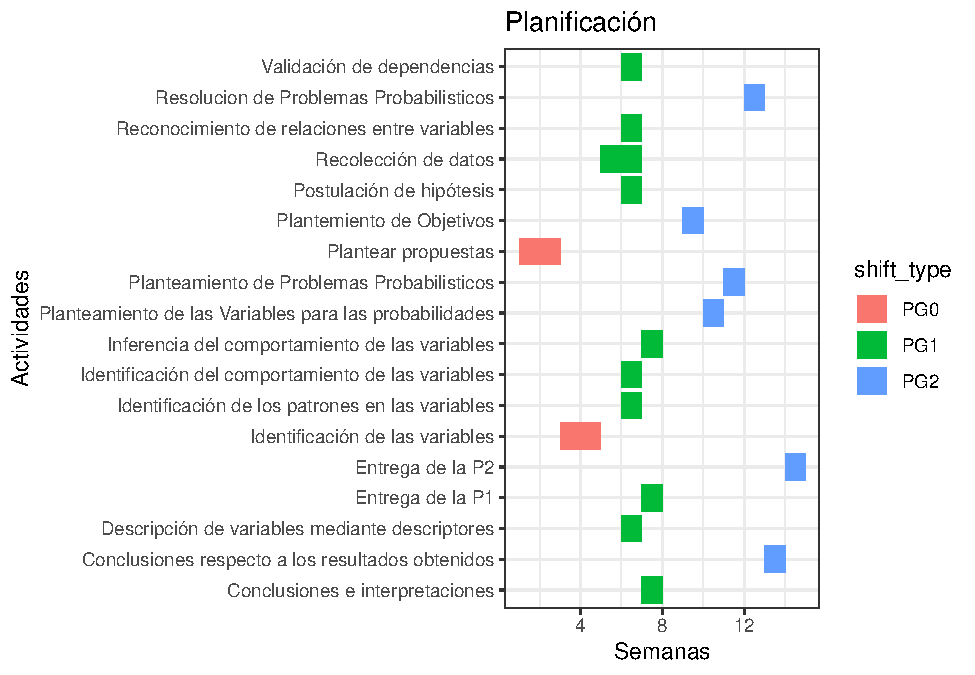
\includegraphics{S7_Informe_files/figure-latex/unnamed-chunk-2-1.pdf}

\hypertarget{datos}{%
\section{2) Datos}\label{datos}}

\hypertarget{proceso-de-recolecciuxf3n-de-datos}{%
\subsection{Proceso de Recolección de
datos}\label{proceso-de-recolecciuxf3n-de-datos}}

La data en bruto utilizada para este proyecto se extrajo de los archivos
del primero semestre del 2021 de la
\href{https://www.datosabiertos.gob.pe/}{Plataforma Nacional de Datos
Abierto del Peru} del
\href{https://www.datosabiertos.gob.pe/dataset/sistema-de-informaci\%C3\%B3n-del-estado-nutricional-de-ni\%C3\%B1os-y-gestantes-per\%C3\%BA-inscenan-instituto}{Sistema
de información del Estado Nutricional de niños y gestantes Perú -
INS/CENAN}

Esta base de datos es una fuente secundaria recopilada por el INS de la
data de Historias Clínicas de los Establecimiento de Salud del Perú
sobre el estado nutricional de niños menores de cinco años y mujeres
gestantes.

El uso de este método de recolección nos permite afrontar el problema de
recolección de data sobre una población extremadamente grande con éxito.

\hypertarget{poblaciuxf3n-muestra-y-muestreo}{%
\subsection{Población, muestra y
muestreo}\label{poblaciuxf3n-muestra-y-muestreo}}

\hypertarget{poblaciuxf3n-de-estudio}{%
\subsubsection{Población de estudio}\label{poblaciuxf3n-de-estudio}}

Este trabajo busca estudiar y establecer una relación entre dos
poblaciones distintas. Estas corresponden a:

\begin{itemize}
\tightlist
\item
  Mujeres gestantes en el primer semestre del 2021
\item
  Niños menores de 5 años en el primer semestre del 2021
\end{itemize}

\hypertarget{muestra-y-muestreo}{%
\subsubsection{Muestra y Muestreo}\label{muestra-y-muestreo}}

Para dicho fin, la muestra seleccionada de estas poblaciones corresponde
a las Mujeres gestantes y Niños menores de 5 años que fueron atendidas y
registradas en el SIEN (Sistema de Información del Estado Nutricional)
durante el primer semestre del 2021. El tamaño de este muestreo en los
niños corresponde a un total de 942869 observaciones, mientras que para
las madres gestantes el numero de observaciones es 190429.

El tipo de muestreo utilizado para la construcción de esta base de datos
es por conveniencia. Ello se debe a que se ha recolectado únicamente
información sobre las mujeres gestantes y niños que han recibido
atención medica en un centro de salud. Esto podría potencialmente
representar un sesgo en nuestro estudio, sin embargo el numero de
observaciones realizadas es lo suficientemente elevado para que se
considera que esto no sea un problema y se conserve un alto grado de
representatividad.

\hypertarget{variables}{%
\subsection{Variables}\label{variables}}

Se tomó en cuenta las siguientes variables.

Con respecto a la población infantil:

\hypertarget{categoricas-nominales}{%
\subsubsection{Categoricas Nominales}\label{categoricas-nominales}}

\begin{itemize}
\tightlist
\item
  DIRESA: Lugar de procedencia del individuo - Restricción: Tiene que
  ser una región del Perú
\end{itemize}

\hypertarget{categoricas-ordinales}{%
\subsubsection{Categoricas Ordinales}\label{categoricas-ordinales}}

\begin{itemize}
\tightlist
\item
  Estado Nutricional Agudo - Restricción: Valor tiene que ser
  {[}``D.Aguda'',``Normal'',``Obesidad'',``Sobrepeso''{]}
\item
  Estado Nutricional Crónica - Restricción: Valor tiene que ser
  {[}``D.Crónica'',``Normal'',``Obesidad'',``Sobrepeso''{]}
\item
  Estado Nutricional Global - Restricción: Valor tiene que ser
  {[}``D.Global'',``Normal'',``Obesidad'',``Sobrepeso''{]}
\end{itemize}

Para las madres gestantes:

\hypertarget{categoricas-nominales-1}{%
\subsubsection{Categoricas Nominales}\label{categoricas-nominales-1}}

\begin{itemize}
\tightlist
\item
  DIRESA: Lugar de procedencia de la madre - Restricción: Tiene que ser
  una región del Perú
\end{itemize}

\hypertarget{categoricas-ordinales-1}{%
\subsubsection{Categoricas Ordinales}\label{categoricas-ordinales-1}}

\begin{itemize}
\tightlist
\item
  Tipo de Ganancia de Peso- Restricción: Valor tiene que ser
  {[}``Déficit'',``Normal'',``Sobrepeso'',``No Evaluado''{]}
\end{itemize}

\hypertarget{limpieza-de-base-de-datos}{%
\subsection{Limpieza de Base de Datos}\label{limpieza-de-base-de-datos}}

La base de datos original del INS se encuentra dividida en múltiples
archivos csv por DIRESAs. Para trabajar con esta data fue necesario
unificarla en dos archivos: PT\_Niños.csv y PT\_Gestantes.csv. Por estar
en español, las tildes ocasionaban problemas con los paquetes
utilizados, fue necesario usar la función iconv en las columnas con
tildes para convertir sus strings en caracteres ASCII, eliminando así
las tildes.

\begin{Shaded}
\begin{Highlighting}[]
\DocumentationTok{\#\# CARGA DE ARCHIVOS}
\CommentTok{\# Niños}
\NormalTok{regiones }\OtherTok{=} \FunctionTok{c}\NormalTok{(}\StringTok{"AMAZONAS"}\NormalTok{, }\StringTok{"ANCASH"}\NormalTok{, }\StringTok{"APURIMAC"}\NormalTok{, }\StringTok{"AREQUIPA"}\NormalTok{, }\StringTok{"AYACUCHO"}\NormalTok{, }\StringTok{"CAJAMARCA"}\NormalTok{, }\StringTok{"CALLAO"}\NormalTok{, }\StringTok{"CUSCO"}\NormalTok{, }\StringTok{"HUANCAVELICA"}\NormalTok{, }\StringTok{"HUANUCO"}\NormalTok{, }\StringTok{"ICA"}\NormalTok{, }\StringTok{"JUNIN"}\NormalTok{, }\StringTok{"LA LIBERTAD"}\NormalTok{, }\StringTok{"LAMBAYEQUE"}\NormalTok{, }\StringTok{"LIMA DIRIS CENTRO"}\NormalTok{, }\StringTok{"LIMA DIRIS ESTE"}\NormalTok{, }\StringTok{"LIMA DIRIS NORTE"}\NormalTok{, }\StringTok{"LIMA DIRIS SUR"}\NormalTok{, }\StringTok{"LIMA"}\NormalTok{, }\StringTok{"LORETO"}\NormalTok{, }\StringTok{"MADRE DE DIOS"}\NormalTok{, }\StringTok{"MOQUEGUA"}\NormalTok{, }\StringTok{"PASCO"}\NormalTok{, }\StringTok{"PIURA"}\NormalTok{, }\StringTok{"PUNO"}\NormalTok{, }\StringTok{"SAN MARTIN"}\NormalTok{, }\StringTok{"TACNA"}\NormalTok{, }\StringTok{"TUMBES"}\NormalTok{, }\StringTok{"UCAYALI"}\NormalTok{)}

\FunctionTok{rm}\NormalTok{(DFNd)}
\end{Highlighting}
\end{Shaded}

\begin{verbatim}
## Warning in rm(DFNd): objeto 'DFNd' no encontrado
\end{verbatim}

\begin{Shaded}
\begin{Highlighting}[]
\NormalTok{DFNd }\OtherTok{\textless{}{-}} \FunctionTok{data.frame}\NormalTok{()}
\ControlFlowTok{for}\NormalTok{ (r }\ControlFlowTok{in}\NormalTok{ regiones) \{}
\NormalTok{  temp}\OtherTok{\textless{}{-}} \FunctionTok{read\_csv}\NormalTok{(}\FunctionTok{paste}\NormalTok{(}\StringTok{"HIS\_Niños\_ISem/PT/Niños "}\NormalTok{,r,}\StringTok{".csv"}\NormalTok{,}\AttributeTok{sep=}\StringTok{""}\NormalTok{))}
\NormalTok{  DFNd }\OtherTok{\textless{}{-}} \FunctionTok{rbind}\NormalTok{(DFNd,temp)}
\NormalTok{\}}
\end{Highlighting}
\end{Shaded}

\begin{verbatim}
## Rows: 39862 Columns: 43
## -- Column specification --------------------------------------------------------
## Delimiter: ","
## chr (24): Diresa, Red, Microred, EESS, Dpto_EESS, Prov_EESS, Dist_EESS, Fech...
## dbl (18): Renipress, EdadMeses, UbigeoPN, Juntos, SIS, Pin, Qaliwarma, Peso,...
## lgl  (1): Alerta
## 
## i Use `spec()` to retrieve the full column specification for this data.
## i Specify the column types or set `show_col_types = FALSE` to quiet this message.
## Rows: 35001 Columns: 43
## -- Column specification --------------------------------------------------------
## Delimiter: ","
## chr (24): Diresa, Red, Microred, EESS, Dpto_EESS, Prov_EESS, Dist_EESS, Fech...
## dbl (18): Renipress, EdadMeses, UbigeoPN, Juntos, SIS, Pin, Qaliwarma, Peso,...
## lgl  (1): Alerta
## 
## i Use `spec()` to retrieve the full column specification for this data.
## i Specify the column types or set `show_col_types = FALSE` to quiet this message.
## Rows: 14169 Columns: 43
## -- Column specification --------------------------------------------------------
## Delimiter: ","
## chr (24): Diresa, Red, Microred, EESS, Dpto_EESS, Prov_EESS, Dist_EESS, Fech...
## dbl (18): Renipress, EdadMeses, UbigeoPN, Juntos, SIS, Pin, Qaliwarma, Peso,...
## lgl  (1): Alerta
## 
## i Use `spec()` to retrieve the full column specification for this data.
## i Specify the column types or set `show_col_types = FALSE` to quiet this message.
## Rows: 32713 Columns: 43
## -- Column specification --------------------------------------------------------
## Delimiter: ","
## chr (24): Diresa, Red, Microred, EESS, Dpto_EESS, Prov_EESS, Dist_EESS, Fech...
## dbl (18): Renipress, EdadMeses, UbigeoPN, Juntos, SIS, Pin, Qaliwarma, Peso,...
## lgl  (1): Alerta
## 
## i Use `spec()` to retrieve the full column specification for this data.
## i Specify the column types or set `show_col_types = FALSE` to quiet this message.
## Rows: 37121 Columns: 43
## -- Column specification --------------------------------------------------------
## Delimiter: ","
## chr (24): Diresa, Red, Microred, EESS, Dpto_EESS, Prov_EESS, Dist_EESS, Fech...
## dbl (18): Renipress, EdadMeses, UbigeoPN, Juntos, SIS, Pin, Qaliwarma, Peso,...
## lgl  (1): Alerta
## 
## i Use `spec()` to retrieve the full column specification for this data.
## i Specify the column types or set `show_col_types = FALSE` to quiet this message.
## Rows: 100431 Columns: 43
## -- Column specification --------------------------------------------------------
## Delimiter: ","
## chr (24): Diresa, Red, Microred, EESS, Dpto_EESS, Prov_EESS, Dist_EESS, Fech...
## dbl (18): Renipress, EdadMeses, UbigeoPN, Juntos, SIS, Pin, Qaliwarma, Peso,...
## lgl  (1): Alerta
## 
## i Use `spec()` to retrieve the full column specification for this data.
## i Specify the column types or set `show_col_types = FALSE` to quiet this message.
## Rows: 12046 Columns: 43
## -- Column specification --------------------------------------------------------
## Delimiter: ","
## chr (24): Diresa, Red, Microred, EESS, Dpto_EESS, Prov_EESS, Dist_EESS, Fech...
## dbl (18): Renipress, EdadMeses, UbigeoPN, Juntos, SIS, Pin, Qaliwarma, Peso,...
## lgl  (1): Alerta
## 
## i Use `spec()` to retrieve the full column specification for this data.
## i Specify the column types or set `show_col_types = FALSE` to quiet this message.
## Rows: 50072 Columns: 43
## -- Column specification --------------------------------------------------------
## Delimiter: ","
## chr (24): Diresa, Red, Microred, EESS, Dpto_EESS, Prov_EESS, Dist_EESS, Fech...
## dbl (18): Renipress, EdadMeses, UbigeoPN, Juntos, SIS, Pin, Qaliwarma, Peso,...
## lgl  (1): Alerta
## 
## i Use `spec()` to retrieve the full column specification for this data.
## i Specify the column types or set `show_col_types = FALSE` to quiet this message.
## Rows: 18417 Columns: 43
## -- Column specification --------------------------------------------------------
## Delimiter: ","
## chr (24): Diresa, Red, Microred, EESS, Dpto_EESS, Prov_EESS, Dist_EESS, Fech...
## dbl (18): Renipress, EdadMeses, UbigeoPN, Juntos, SIS, Pin, Qaliwarma, Peso,...
## lgl  (1): Alerta
## 
## i Use `spec()` to retrieve the full column specification for this data.
## i Specify the column types or set `show_col_types = FALSE` to quiet this message.
## Rows: 43044 Columns: 43
## -- Column specification --------------------------------------------------------
## Delimiter: ","
## chr (23): Diresa, Red, Microred, EESS, Dpto_EESS, Prov_EESS, Dist_EESS, Fech...
## dbl (19): Renipress, EdadMeses, UbigeoPN, Juntos, SIS, Pin, Qaliwarma, Peso,...
## lgl  (1): Alerta
## 
## i Use `spec()` to retrieve the full column specification for this data.
## i Specify the column types or set `show_col_types = FALSE` to quiet this message.
## Rows: 20604 Columns: 43
## -- Column specification --------------------------------------------------------
## Delimiter: ","
## chr (23): Diresa, Red, Microred, EESS, Dpto_EESS, Prov_EESS, Dist_EESS, Fech...
## dbl (19): Renipress, EdadMeses, UbigeoPN, Juntos, SIS, Pin, Qaliwarma, Peso,...
## lgl  (1): Alerta
## 
## i Use `spec()` to retrieve the full column specification for this data.
## i Specify the column types or set `show_col_types = FALSE` to quiet this message.
## Rows: 22776 Columns: 43
## -- Column specification --------------------------------------------------------
## Delimiter: ","
## chr (23): Diresa, Red, Microred, EESS, Dpto_EESS, Prov_EESS, Dist_EESS, Fech...
## dbl (19): Renipress, EdadMeses, UbigeoPN, Juntos, SIS, Pin, Qaliwarma, Peso,...
## lgl  (1): Alerta
## 
## i Use `spec()` to retrieve the full column specification for this data.
## i Specify the column types or set `show_col_types = FALSE` to quiet this message.
## Rows: 42842 Columns: 43
## -- Column specification --------------------------------------------------------
## Delimiter: ","
## chr (23): Diresa, Red, Microred, EESS, Dpto_EESS, Prov_EESS, Dist_EESS, Fech...
## dbl (19): Renipress, EdadMeses, UbigeoPN, Juntos, SIS, Pin, Qaliwarma, Peso,...
## lgl  (1): Alerta
## 
## i Use `spec()` to retrieve the full column specification for this data.
## i Specify the column types or set `show_col_types = FALSE` to quiet this message.
## Rows: 21857 Columns: 43
## -- Column specification --------------------------------------------------------
## Delimiter: ","
## chr (23): Diresa, Red, Microred, EESS, Dpto_EESS, Prov_EESS, Dist_EESS, Fech...
## dbl (19): Renipress, EdadMeses, UbigeoPN, Juntos, SIS, Pin, Qaliwarma, Peso,...
## lgl  (1): Alerta
## 
## i Use `spec()` to retrieve the full column specification for this data.
## i Specify the column types or set `show_col_types = FALSE` to quiet this message.
## Rows: 16087 Columns: 43
## -- Column specification --------------------------------------------------------
## Delimiter: ","
## chr (23): Diresa, Red, Microred, EESS, Dpto_EESS, Prov_EESS, Dist_EESS, Fech...
## dbl (19): Renipress, EdadMeses, UbigeoPN, Juntos, SIS, Pin, Qaliwarma, Peso,...
## lgl  (1): Alerta
## 
## i Use `spec()` to retrieve the full column specification for this data.
## i Specify the column types or set `show_col_types = FALSE` to quiet this message.
## Rows: 18193 Columns: 43
## -- Column specification --------------------------------------------------------
## Delimiter: ","
## chr (23): Diresa, Red, Microred, EESS, Dpto_EESS, Prov_EESS, Dist_EESS, Fech...
## dbl (19): Renipress, EdadMeses, UbigeoPN, Juntos, SIS, Pin, Qaliwarma, Peso,...
## lgl  (1): Alerta
## 
## i Use `spec()` to retrieve the full column specification for this data.
## i Specify the column types or set `show_col_types = FALSE` to quiet this message.
## Rows: 37757 Columns: 43
## -- Column specification --------------------------------------------------------
## Delimiter: ","
## chr (23): Diresa, Red, Microred, EESS, Dpto_EESS, Prov_EESS, Dist_EESS, Fech...
## dbl (19): Renipress, EdadMeses, UbigeoPN, Juntos, SIS, Pin, Qaliwarma, Peso,...
## lgl  (1): Alerta
## 
## i Use `spec()` to retrieve the full column specification for this data.
## i Specify the column types or set `show_col_types = FALSE` to quiet this message.
## Rows: 19344 Columns: 43
## -- Column specification --------------------------------------------------------
## Delimiter: ","
## chr (23): Diresa, Red, Microred, EESS, Dpto_EESS, Prov_EESS, Dist_EESS, Fech...
## dbl (19): Renipress, EdadMeses, UbigeoPN, Juntos, SIS, Pin, Qaliwarma, Peso,...
## lgl  (1): Alerta
## 
## i Use `spec()` to retrieve the full column specification for this data.
## i Specify the column types or set `show_col_types = FALSE` to quiet this message.
## Rows: 29140 Columns: 43
## -- Column specification --------------------------------------------------------
## Delimiter: ","
## chr (23): Diresa, Red, Microred, EESS, Dpto_EESS, Prov_EESS, Dist_EESS, Fech...
## dbl (19): Renipress, EdadMeses, UbigeoPN, Juntos, SIS, Pin, Qaliwarma, Peso,...
## lgl  (1): Alerta
## 
## i Use `spec()` to retrieve the full column specification for this data.
## i Specify the column types or set `show_col_types = FALSE` to quiet this message.
## Rows: 75628 Columns: 43
## -- Column specification --------------------------------------------------------
## Delimiter: ","
## chr (23): Diresa, Red, Microred, EESS, Dpto_EESS, Prov_EESS, Dist_EESS, Fech...
## dbl (19): Renipress, EdadMeses, UbigeoPN, Juntos, SIS, Pin, Qaliwarma, Peso,...
## lgl  (1): Alerta
## 
## i Use `spec()` to retrieve the full column specification for this data.
## i Specify the column types or set `show_col_types = FALSE` to quiet this message.
## Rows: 9883 Columns: 43
## -- Column specification --------------------------------------------------------
## Delimiter: ","
## chr (23): Diresa, Red, Microred, EESS, Dpto_EESS, Prov_EESS, Dist_EESS, Fech...
## dbl (19): Renipress, EdadMeses, UbigeoPN, Juntos, SIS, Pin, Qaliwarma, Peso,...
## lgl  (1): Alerta
## 
## i Use `spec()` to retrieve the full column specification for this data.
## i Specify the column types or set `show_col_types = FALSE` to quiet this message.
## Rows: 4633 Columns: 43
## -- Column specification --------------------------------------------------------
## Delimiter: ","
## chr (23): Diresa, Red, Microred, EESS, Dpto_EESS, Prov_EESS, Dist_EESS, Fech...
## dbl (19): Renipress, EdadMeses, UbigeoPN, Juntos, SIS, Pin, Qaliwarma, Peso,...
## lgl  (1): Alerta
## 
## i Use `spec()` to retrieve the full column specification for this data.
## i Specify the column types or set `show_col_types = FALSE` to quiet this message.
## Rows: 12280 Columns: 43
## -- Column specification --------------------------------------------------------
## Delimiter: ","
## chr (23): Diresa, Red, Microred, EESS, Dpto_EESS, Prov_EESS, Dist_EESS, Fech...
## dbl (19): Renipress, EdadMeses, UbigeoPN, Juntos, SIS, Pin, Qaliwarma, Peso,...
## lgl  (1): Alerta
## 
## i Use `spec()` to retrieve the full column specification for this data.
## i Specify the column types or set `show_col_types = FALSE` to quiet this message.
## Rows: 90948 Columns: 43
## -- Column specification --------------------------------------------------------
## Delimiter: ","
## chr (23): Diresa, Red, Microred, EESS, Dpto_EESS, Prov_EESS, Dist_EESS, Fech...
## dbl (19): Renipress, EdadMeses, UbigeoPN, Juntos, SIS, Pin, Qaliwarma, Peso,...
## lgl  (1): Alerta
## 
## i Use `spec()` to retrieve the full column specification for this data.
## i Specify the column types or set `show_col_types = FALSE` to quiet this message.
## Rows: 46607 Columns: 43
## -- Column specification --------------------------------------------------------
## Delimiter: ","
## chr (23): Diresa, Red, Microred, EESS, Dpto_EESS, Prov_EESS, Dist_EESS, Fech...
## dbl (19): Renipress, EdadMeses, UbigeoPN, Juntos, SIS, Pin, Qaliwarma, Peso,...
## lgl  (1): Alerta
## 
## i Use `spec()` to retrieve the full column specification for this data.
## i Specify the column types or set `show_col_types = FALSE` to quiet this message.
## Rows: 52613 Columns: 43
## -- Column specification --------------------------------------------------------
## Delimiter: ","
## chr (23): Diresa, Red, Microred, EESS, Dpto_EESS, Prov_EESS, Dist_EESS, Fech...
## dbl (19): Renipress, EdadMeses, UbigeoPN, Juntos, SIS, Pin, Qaliwarma, Peso,...
## lgl  (1): Alerta
## 
## i Use `spec()` to retrieve the full column specification for this data.
## i Specify the column types or set `show_col_types = FALSE` to quiet this message.
## Rows: 9168 Columns: 43
## -- Column specification --------------------------------------------------------
## Delimiter: ","
## chr (23): Diresa, Red, Microred, EESS, Dpto_EESS, Prov_EESS, Dist_EESS, Fech...
## dbl (19): Renipress, EdadMeses, UbigeoPN, Juntos, SIS, Pin, Qaliwarma, Peso,...
## lgl  (1): Alerta
## 
## i Use `spec()` to retrieve the full column specification for this data.
## i Specify the column types or set `show_col_types = FALSE` to quiet this message.
## Rows: 7370 Columns: 43
## -- Column specification --------------------------------------------------------
## Delimiter: ","
## chr (23): Diresa, Red, Microred, EESS, Dpto_EESS, Prov_EESS, Dist_EESS, Fech...
## dbl (19): Renipress, EdadMeses, UbigeoPN, Juntos, SIS, Pin, Qaliwarma, Peso,...
## lgl  (1): Alerta
## 
## i Use `spec()` to retrieve the full column specification for this data.
## i Specify the column types or set `show_col_types = FALSE` to quiet this message.
## Rows: 22263 Columns: 43
## -- Column specification --------------------------------------------------------
## Delimiter: ","
## chr (23): Diresa, Red, Microred, EESS, Dpto_EESS, Prov_EESS, Dist_EESS, Fech...
## dbl (19): Renipress, EdadMeses, UbigeoPN, Juntos, SIS, Pin, Qaliwarma, Peso,...
## lgl  (1): Alerta
## 
## i Use `spec()` to retrieve the full column specification for this data.
## i Specify the column types or set `show_col_types = FALSE` to quiet this message.
\end{verbatim}

\begin{Shaded}
\begin{Highlighting}[]
\CommentTok{\# Gestantes }
\NormalTok{regiones }\OtherTok{=} \FunctionTok{c}\NormalTok{(}\StringTok{"Amazonas"}\NormalTok{,}\StringTok{"Ancash"}\NormalTok{,}\StringTok{"Andahuaylas"}\NormalTok{,}\StringTok{"Apurimac"}\NormalTok{,}\StringTok{"Ayacucho"}\NormalTok{,}\StringTok{"Cusco"}\NormalTok{,}\StringTok{"Cutervo"}\NormalTok{,}\StringTok{"Huancavelica"}\NormalTok{,}\StringTok{"Ica"}\NormalTok{,}\StringTok{"Jaen"}\NormalTok{,}\StringTok{"Junin"}\NormalTok{,}\StringTok{"La Libertad"}\NormalTok{,}\StringTok{"Lambayeque"}\NormalTok{,}\StringTok{"Lima Centro"}\NormalTok{,}\StringTok{"Lima Este"}\NormalTok{,}\StringTok{"Lima Sur"}\NormalTok{,}\StringTok{"Lima"}\NormalTok{,}\StringTok{"Loreto"}\NormalTok{,}\StringTok{"Madre De Dios"}\NormalTok{,}\StringTok{"Pasco"}\NormalTok{,}\StringTok{"Piura"}\NormalTok{,}\StringTok{"Puno"}\NormalTok{,}\StringTok{"Sullana"}\NormalTok{,}\StringTok{"Tacna"}\NormalTok{,}\StringTok{"Tumbes"}\NormalTok{)}

\FunctionTok{rm}\NormalTok{(DFG)}
\end{Highlighting}
\end{Shaded}

\begin{verbatim}
## Warning in rm(DFG): objeto 'DFG' no encontrado
\end{verbatim}

\begin{Shaded}
\begin{Highlighting}[]
\NormalTok{DFGd }\OtherTok{\textless{}{-}} \FunctionTok{data.frame}\NormalTok{()}
\ControlFlowTok{for}\NormalTok{ (r }\ControlFlowTok{in}\NormalTok{ regiones) \{}
\NormalTok{  temp}\OtherTok{\textless{}{-}} \FunctionTok{read\_csv}\NormalTok{(}\FunctionTok{paste}\NormalTok{(}\StringTok{"SIEN\_Gestantes\_ISem/PT/Gestantes "}\NormalTok{,r,}\StringTok{".csv"}\NormalTok{,}\AttributeTok{sep=}\StringTok{""}\NormalTok{))}
\NormalTok{  DFGd }\OtherTok{\textless{}{-}} \FunctionTok{rbind}\NormalTok{(DFGd,temp)}
\NormalTok{\}}
\end{Highlighting}
\end{Shaded}

\begin{verbatim}
## Warning: One or more parsing issues, see `problems()` for details
\end{verbatim}

\begin{verbatim}
## Rows: 16118 Columns: 20
## -- Column specification --------------------------------------------------------
## Delimiter: ","
## chr (12): DIRESA, RED, MICRORED, EESS, Fecha, Tipo_Embarazo, UBIGEO, Provinc...
## dbl  (8): RENIPRESS, Edad, Edad_Gestacional, Peso, Talla, PPG, Altitud_Dist,...
## 
## i Use `spec()` to retrieve the full column specification for this data.
## i Specify the column types or set `show_col_types = FALSE` to quiet this message.
\end{verbatim}

\begin{verbatim}
## Warning: One or more parsing issues, see `problems()` for details
\end{verbatim}

\begin{verbatim}
## Rows: 9365 Columns: 20
## -- Column specification --------------------------------------------------------
## Delimiter: ","
## chr (12): DIRESA, RED, MICRORED, EESS, Fecha, Tipo_Embarazo, UBIGEO, Provinc...
## dbl  (8): RENIPRESS, Edad, Edad_Gestacional, Peso, Talla, PPG, Altitud_Dist,...
## 
## i Use `spec()` to retrieve the full column specification for this data.
## i Specify the column types or set `show_col_types = FALSE` to quiet this message.
## Rows: 2233 Columns: 20
## -- Column specification --------------------------------------------------------
## Delimiter: ","
## chr (12): DIRESA, RED, MICRORED, EESS, Fecha, Tipo_Embarazo, UBIGEO, Provinc...
## dbl  (8): RENIPRESS, Edad, Edad_Gestacional, Peso, Talla, PPG, Altitud_Dist,...
## 
## i Use `spec()` to retrieve the full column specification for this data.
## i Specify the column types or set `show_col_types = FALSE` to quiet this message.
## Rows: 4069 Columns: 20
## -- Column specification --------------------------------------------------------
## Delimiter: ","
## chr (12): DIRESA, RED, MICRORED, EESS, Fecha, Tipo_Embarazo, UBIGEO, Provinc...
## dbl  (8): RENIPRESS, Edad, Edad_Gestacional, Peso, Talla, PPG, Altitud_Dist,...
## 
## i Use `spec()` to retrieve the full column specification for this data.
## i Specify the column types or set `show_col_types = FALSE` to quiet this message.
## Rows: 9635 Columns: 20
## -- Column specification --------------------------------------------------------
## Delimiter: ","
## chr (12): DIRESA, RED, MICRORED, EESS, Fecha, Tipo_Embarazo, UBIGEO, Provinc...
## dbl  (8): RENIPRESS, Edad, Edad_Gestacional, Peso, Talla, PPG, Altitud_Dist,...
## 
## i Use `spec()` to retrieve the full column specification for this data.
## i Specify the column types or set `show_col_types = FALSE` to quiet this message.
\end{verbatim}

\begin{verbatim}
## Warning: One or more parsing issues, see `problems()` for details
\end{verbatim}

\begin{verbatim}
## Rows: 17624 Columns: 20
## -- Column specification --------------------------------------------------------
## Delimiter: ","
## chr (12): DIRESA, RED, MICRORED, EESS, Fecha, Tipo_Embarazo, UBIGEO, Provinc...
## dbl  (8): RENIPRESS, Edad, Edad_Gestacional, Peso, Talla, PPG, Altitud_Dist,...
## 
## i Use `spec()` to retrieve the full column specification for this data.
## i Specify the column types or set `show_col_types = FALSE` to quiet this message.
## Rows: 2013 Columns: 20
## -- Column specification --------------------------------------------------------
## Delimiter: ","
## chr (12): DIRESA, RED, MICRORED, EESS, Fecha, Tipo_Embarazo, UBIGEO, Provinc...
## dbl  (8): RENIPRESS, Edad, Edad_Gestacional, Peso, Talla, PPG, Altitud_Dist,...
## 
## i Use `spec()` to retrieve the full column specification for this data.
## i Specify the column types or set `show_col_types = FALSE` to quiet this message.
\end{verbatim}

\begin{verbatim}
## Warning: One or more parsing issues, see `problems()` for details
\end{verbatim}

\begin{verbatim}
## Rows: 6256 Columns: 20
## -- Column specification --------------------------------------------------------
## Delimiter: ","
## chr (12): DIRESA, RED, MICRORED, EESS, Fecha, Tipo_Embarazo, UBIGEO, Provinc...
## dbl  (8): RENIPRESS, Edad, Edad_Gestacional, Peso, Talla, PPG, Altitud_Dist,...
## 
## i Use `spec()` to retrieve the full column specification for this data.
## i Specify the column types or set `show_col_types = FALSE` to quiet this message.
## Rows: 8673 Columns: 20
## -- Column specification --------------------------------------------------------
## Delimiter: ","
## chr (11): DIRESA, RED, MICRORED, EESS, Fecha, Tipo_Embarazo, Provincia, Dist...
## dbl  (9): RENIPRESS, Edad, Edad_Gestacional, Peso, Talla, PPG, UBIGEO, Altit...
## 
## i Use `spec()` to retrieve the full column specification for this data.
## i Specify the column types or set `show_col_types = FALSE` to quiet this message.
\end{verbatim}

\begin{verbatim}
## Warning: One or more parsing issues, see `problems()` for details
\end{verbatim}

\begin{verbatim}
## Rows: 5559 Columns: 20
## -- Column specification --------------------------------------------------------
## Delimiter: ","
## chr (12): DIRESA, RED, MICRORED, EESS, Fecha, Tipo_Embarazo, UBIGEO, Provinc...
## dbl  (8): RENIPRESS, Edad, Edad_Gestacional, Peso, Talla, PPG, Altitud_Dist,...
## 
## i Use `spec()` to retrieve the full column specification for this data.
## i Specify the column types or set `show_col_types = FALSE` to quiet this message.
## Rows: 15557 Columns: 20
## -- Column specification --------------------------------------------------------
## Delimiter: ","
## chr (11): DIRESA, RED, MICRORED, EESS, Fecha, Tipo_Embarazo, Provincia, Dist...
## dbl  (9): RENIPRESS, Edad, Edad_Gestacional, Peso, Talla, PPG, UBIGEO, Altit...
## 
## i Use `spec()` to retrieve the full column specification for this data.
## i Specify the column types or set `show_col_types = FALSE` to quiet this message.
## Rows: 10452 Columns: 20
## -- Column specification --------------------------------------------------------
## Delimiter: ","
## chr (12): DIRESA, RED, MICRORED, EESS, Fecha, Tipo_Embarazo, Provincia, Dist...
## dbl  (8): RENIPRESS, Edad, Edad_Gestacional, Peso, Talla, PPG, UBIGEO, Altit...
## 
## i Use `spec()` to retrieve the full column specification for this data.
## i Specify the column types or set `show_col_types = FALSE` to quiet this message.
## Rows: 4735 Columns: 20
## -- Column specification --------------------------------------------------------
## Delimiter: ","
## chr (11): DIRESA, RED, MICRORED, EESS, Fecha, Tipo_Embarazo, Provincia, Dist...
## dbl  (9): RENIPRESS, Edad, Edad_Gestacional, Peso, Talla, PPG, UBIGEO, Altit...
## 
## i Use `spec()` to retrieve the full column specification for this data.
## i Specify the column types or set `show_col_types = FALSE` to quiet this message.
\end{verbatim}

\begin{verbatim}
## Warning: One or more parsing issues, see `problems()` for details
\end{verbatim}

\begin{verbatim}
## Rows: 2316 Columns: 20
## -- Column specification --------------------------------------------------------
## Delimiter: ","
## chr (11): DIRESA, RED, MICRORED, EESS, Fecha, Tipo_Embarazo, Provincia, Dist...
## dbl  (9): RENIPRESS, Edad, Edad_Gestacional, Peso, Talla, PPG, UBIGEO, Altit...
## 
## i Use `spec()` to retrieve the full column specification for this data.
## i Specify the column types or set `show_col_types = FALSE` to quiet this message.
## Rows: 4459 Columns: 20
## -- Column specification --------------------------------------------------------
## Delimiter: ","
## chr (11): DIRESA, RED, MICRORED, EESS, Fecha, Tipo_Embarazo, Provincia, Dist...
## dbl  (9): RENIPRESS, Edad, Edad_Gestacional, Peso, Talla, PPG, UBIGEO, Altit...
## 
## i Use `spec()` to retrieve the full column specification for this data.
## i Specify the column types or set `show_col_types = FALSE` to quiet this message.
## Rows: 9879 Columns: 20
## -- Column specification --------------------------------------------------------
## Delimiter: ","
## chr (11): DIRESA, RED, MICRORED, EESS, Fecha, Tipo_Embarazo, Provincia, Dist...
## dbl  (9): RENIPRESS, Edad, Edad_Gestacional, Peso, Talla, PPG, UBIGEO, Altit...
## 
## i Use `spec()` to retrieve the full column specification for this data.
## i Specify the column types or set `show_col_types = FALSE` to quiet this message.
## Rows: 7161 Columns: 20
## -- Column specification --------------------------------------------------------
## Delimiter: ","
## chr (11): DIRESA, RED, MICRORED, EESS, Fecha, Tipo_Embarazo, Provincia, Dist...
## dbl  (9): RENIPRESS, Edad, Edad_Gestacional, Peso, Talla, PPG, UBIGEO, Altit...
## 
## i Use `spec()` to retrieve the full column specification for this data.
## i Specify the column types or set `show_col_types = FALSE` to quiet this message.
\end{verbatim}

\begin{verbatim}
## Warning: One or more parsing issues, see `problems()` for details
\end{verbatim}

\begin{verbatim}
## Rows: 16630 Columns: 20
## -- Column specification --------------------------------------------------------
## Delimiter: ","
## chr (11): DIRESA, RED, MICRORED, EESS, Fecha, Tipo_Embarazo, Provincia, Dist...
## dbl  (9): RENIPRESS, Edad, Edad_Gestacional, Peso, Talla, PPG, UBIGEO, Altit...
## 
## i Use `spec()` to retrieve the full column specification for this data.
## i Specify the column types or set `show_col_types = FALSE` to quiet this message.
## Rows: 3919 Columns: 20
## -- Column specification --------------------------------------------------------
## Delimiter: ","
## chr (11): DIRESA, RED, MICRORED, EESS, Fecha, Tipo_Embarazo, Provincia, Dist...
## dbl  (9): RENIPRESS, Edad, Edad_Gestacional, Peso, Talla, PPG, UBIGEO, Altit...
## 
## i Use `spec()` to retrieve the full column specification for this data.
## i Specify the column types or set `show_col_types = FALSE` to quiet this message.
## Rows: 2980 Columns: 20
## -- Column specification --------------------------------------------------------
## Delimiter: ","
## chr (12): DIRESA, RED, MICRORED, EESS, Fecha, Tipo_Embarazo, Provincia, Dist...
## dbl  (8): RENIPRESS, Edad, Edad_Gestacional, Peso, Talla, PPG, UBIGEO, Altit...
## 
## i Use `spec()` to retrieve the full column specification for this data.
## i Specify the column types or set `show_col_types = FALSE` to quiet this message.
## Rows: 5117 Columns: 20
## -- Column specification --------------------------------------------------------
## Delimiter: ","
## chr (11): DIRESA, RED, MICRORED, EESS, Fecha, Tipo_Embarazo, Provincia, Dist...
## dbl  (9): RENIPRESS, Edad, Edad_Gestacional, Peso, Talla, PPG, UBIGEO, Altit...
## 
## i Use `spec()` to retrieve the full column specification for this data.
## i Specify the column types or set `show_col_types = FALSE` to quiet this message.
## Rows: 12161 Columns: 20
## -- Column specification --------------------------------------------------------
## Delimiter: ","
## chr (11): DIRESA, RED, MICRORED, EESS, Fecha, Tipo_Embarazo, Provincia, Dist...
## dbl  (9): RENIPRESS, Edad, Edad_Gestacional, Peso, Talla, PPG, UBIGEO, Altit...
## 
## i Use `spec()` to retrieve the full column specification for this data.
## i Specify the column types or set `show_col_types = FALSE` to quiet this message.
## Rows: 7602 Columns: 20
## -- Column specification --------------------------------------------------------
## Delimiter: ","
## chr (12): DIRESA, RED, MICRORED, EESS, Fecha, Tipo_Embarazo, Provincia, Dist...
## dbl  (8): RENIPRESS, Edad, Edad_Gestacional, Peso, Talla, PPG, UBIGEO, Altit...
## 
## i Use `spec()` to retrieve the full column specification for this data.
## i Specify the column types or set `show_col_types = FALSE` to quiet this message.
## Rows: 2416 Columns: 20
## -- Column specification --------------------------------------------------------
## Delimiter: ","
## chr (11): DIRESA, RED, MICRORED, EESS, Fecha, Tipo_Embarazo, Provincia, Dist...
## dbl  (9): RENIPRESS, Edad, Edad_Gestacional, Peso, Talla, PPG, UBIGEO, Altit...
## 
## i Use `spec()` to retrieve the full column specification for this data.
## i Specify the column types or set `show_col_types = FALSE` to quiet this message.
## Rows: 3500 Columns: 20
## -- Column specification --------------------------------------------------------
## Delimiter: ","
## chr (11): DIRESA, RED, MICRORED, EESS, Fecha, Tipo_Embarazo, Provincia, Dist...
## dbl  (9): RENIPRESS, Edad, Edad_Gestacional, Peso, Talla, PPG, UBIGEO, Altit...
## 
## i Use `spec()` to retrieve the full column specification for this data.
## i Specify the column types or set `show_col_types = FALSE` to quiet this message.
\end{verbatim}

\begin{Shaded}
\begin{Highlighting}[]
\DocumentationTok{\#\# LIMPIEZA DE DATA}
\NormalTok{DFNd}\SpecialCharTok{$}\NormalTok{Dx\_TE }\OtherTok{\textless{}{-}} \FunctionTok{iconv}\NormalTok{(DFNd}\SpecialCharTok{$}\NormalTok{Dx\_TE, }\StringTok{"ASCII"}\NormalTok{, }\StringTok{"UTF{-}8"}\NormalTok{, }\AttributeTok{sub=}\StringTok{""}\NormalTok{)}
\NormalTok{DFGd}\SpecialCharTok{$}\NormalTok{Dx\_CLAP }\OtherTok{\textless{}{-}} \FunctionTok{iconv}\NormalTok{(DFGd}\SpecialCharTok{$}\NormalTok{Dx\_CLAP, }\StringTok{"ASCII"}\NormalTok{, }\StringTok{"UTF{-}8"}\NormalTok{, }\AttributeTok{sub=}\StringTok{""}\NormalTok{)}
\DocumentationTok{\#\# ESCRITURA}
\FunctionTok{write\_csv}\NormalTok{(DFNd, }\StringTok{"PT\_Niños.csv"}\NormalTok{)}
\FunctionTok{write\_csv}\NormalTok{(DFGd, }\StringTok{"PT\_Gestantes.csv"}\NormalTok{)}
\end{Highlighting}
\end{Shaded}

\hypertarget{anuxe1lisis-descriptivo}{%
\section{3) Análisis descriptivo}\label{anuxe1lisis-descriptivo}}

\begin{verbatim}
## Rows: 942869 Columns: 43
## -- Column specification --------------------------------------------------------
## Delimiter: ","
## chr (24): Diresa, Red, Microred, EESS, Dpto_EESS, Prov_EESS, Dist_EESS, Fech...
## dbl (18): Renipress, EdadMeses, UbigeoPN, Juntos, SIS, Pin, Qaliwarma, Peso,...
## lgl  (1): Alerta
## 
## i Use `spec()` to retrieve the full column specification for this data.
## i Specify the column types or set `show_col_types = FALSE` to quiet this message.
\end{verbatim}

\begin{verbatim}
## Warning: One or more parsing issues, see `problems()` for details
\end{verbatim}

\begin{verbatim}
## Rows: 190429 Columns: 20
## -- Column specification --------------------------------------------------------
## Delimiter: ","
## chr (12): DIRESA, RED, MICRORED, EESS, Fecha, Tipo_Embarazo, UBIGEO, Provinc...
## dbl  (8): RENIPRESS, Edad, Edad_Gestacional, Peso, Talla, PPG, Altitud_Dist,...
## 
## i Use `spec()` to retrieve the full column specification for this data.
## i Specify the column types or set `show_col_types = FALSE` to quiet this message.
\end{verbatim}

\hypertarget{estado-nutricional-de-los-niuxf1os}{%
\subsection{Estado nutricional de los
niños}\label{estado-nutricional-de-los-niuxf1os}}

El estado nutricional de un niño se evaluó usando tres indicadores:
Talla/Peso, Talla/Edad y Peso/Edad con los cuales se identifico la
desnutrición aguda, crónica y global respectivamente. Para ello se
considera los llamados z-scores, los cuales nos permiten medir cuantas
desviaciones estándar alejadas se encuentra un valor de su punto medio.

\hypertarget{estado-nutricional-agudo}{%
\subsubsection{Estado Nutricional
Agudo}\label{estado-nutricional-agudo}}

El estado nutricional agudo se divide en cuatro categorías: Desnutrición
Aguda cuando el z-score \textless{} (-2), Normal cuando su valor
absoluto es menor a 2, Sobrepeso cuando \textgreater{} 2 y Obesidad
cuando \textgreater3. Los niños en nuestras observaciones han sido
clasificados en base a estos rangos en la columna Dx\_PT.

Utilizando esta data podemos generar un gráfico de barras proporcionales
para poder evaluar la distribución del estado nutricional cronico en
niños por DIRESA.

\begin{verbatim}
## [1] "Minimo: 0.828970331588133"
\end{verbatim}

\begin{verbatim}
## [1] "Maximo: 2.90616718321879"
\end{verbatim}

\begin{verbatim}
## [1] "Desviación Estandar: 0.59763594413174"
\end{verbatim}

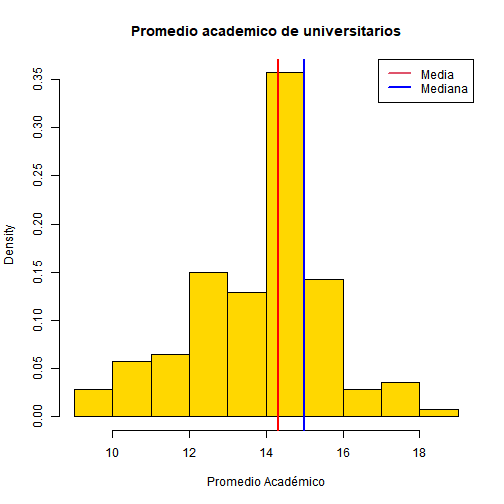
\includegraphics{S7_Informe_files/figure-latex/unnamed-chunk-6-1.pdf} En
el gráfico se observa que la incidencia de Desnutrición Aguda tiene sus
valores máximos en las DIRESAs de Ucayali, Loreto y San Martin en dicho
orden. Todos estos DIRESAs corresponden a la región de la selva. Sin
embargo, es importante destacar que las variaciones entre DIRESAs son
relativamente pequeños. Si calculamos la desviación estándar de la
incidencia por DIRESA, obtendremos que esta es tan solo 0.60.

\hypertarget{estado-nutricional-cronica}{%
\subsubsection{Estado Nutricional
Cronica}\label{estado-nutricional-cronica}}

El estado nutricional crónico se puede dividir utilizando el mismo
criterio en Desnutrición Crónica, Normal, Sobrepeso y Obesidad. Los
niños en nuestras observaciones han sido clasificados en base a estos
rangos en la columna Dx\_TE.

A continuación, se presenta un gráfico de barras proporcionales para
poder evaluar la distribución del estado nutricional crónico en niños
por DIRESA.

\begin{verbatim}
## [1] "Minimo: 3.16317626527051"
\end{verbatim}

\begin{verbatim}
## [1] "Maximo: 23.4077211272194"
\end{verbatim}

\begin{verbatim}
## [1] "Desviación Estandar: 5.71547948631249"
\end{verbatim}

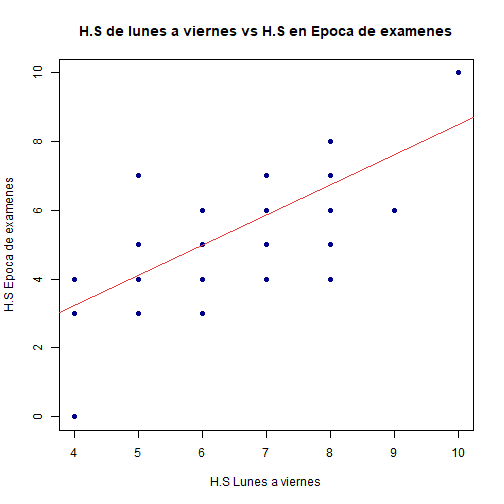
\includegraphics{S7_Informe_files/figure-latex/unnamed-chunk-8-1.pdf} A
diferencia del gráfico previo, se observa que la variación de la
incidencia en Desnutrición Crónica es mayor, teniendo una desviación
estándar de 5.72. Asimismo, en este caso los DIRESAs con mayor
incidencia, estos son Huancavelica, Cajamarca y Amazonas en ese orden
descendente. A diferencia del anterior, aquí la región de la sierra
ocupa los primeros lugares en desnutrición crónica.

\hypertarget{estado-nutricional-global-por-diresa}{%
\subsubsection{Estado Nutricional Global por
DIRESA}\label{estado-nutricional-global-por-diresa}}

Con el mismo criterio, se agrupo la data mostrada en la columna Dx\_PE.
A continuación, se muestra el gráfico de barras proporcionales para la
evaluación de la distribución del estado nutricional global en niños por
DIRESA.

\begin{verbatim}
## [1] "Minimo: 0.567190226876091"
\end{verbatim}

\begin{verbatim}
## [1] "Maximoi: 6.94584016501825"
\end{verbatim}

\begin{verbatim}
## [1] "Desviación Estandar: 1.47255898931176"
\end{verbatim}

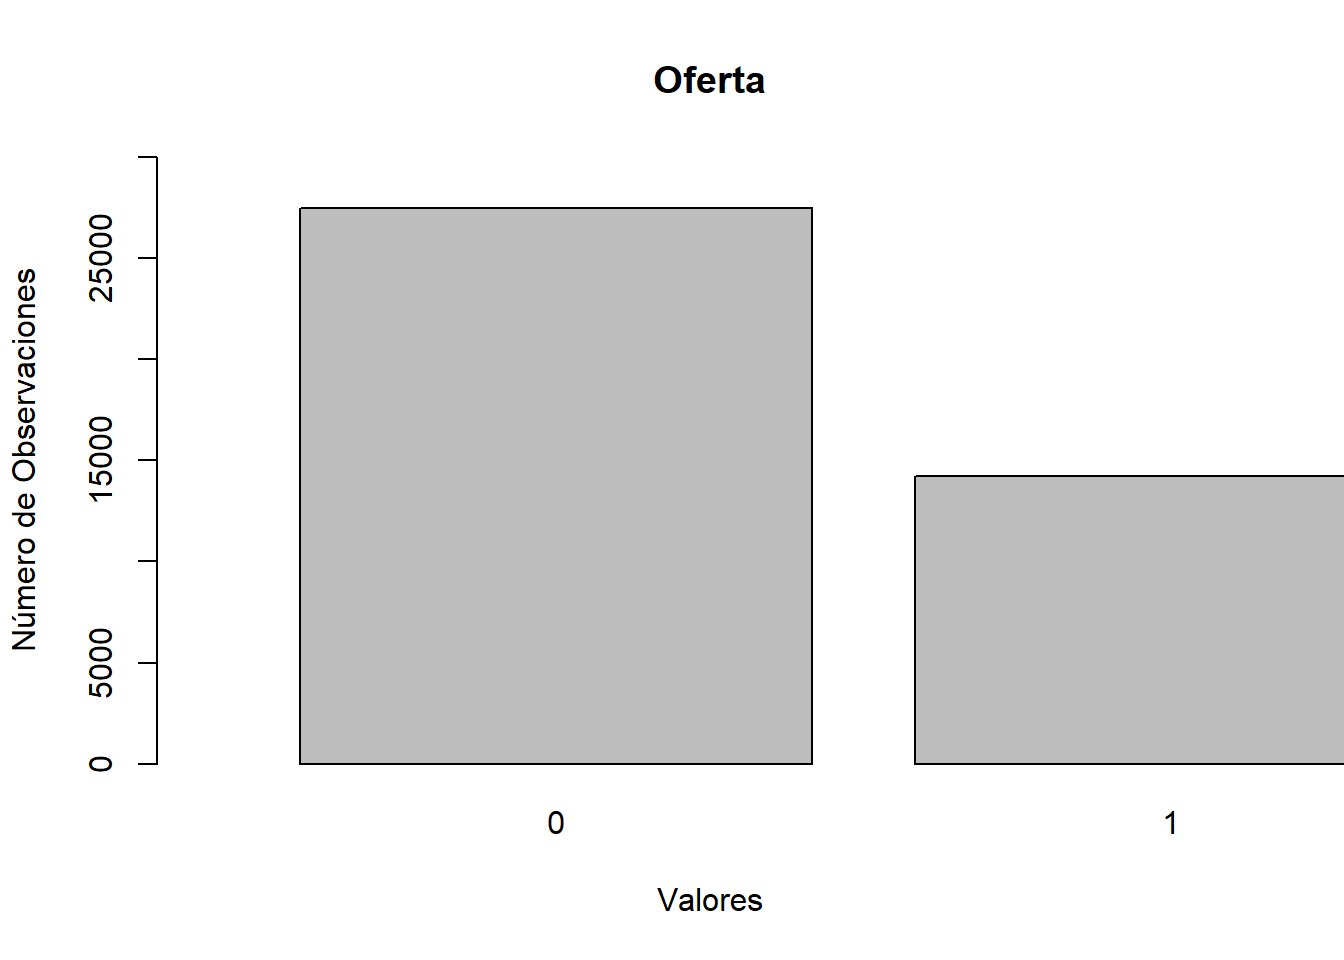
\includegraphics{S7_Informe_files/figure-latex/unnamed-chunk-10-1.pdf}
Como se observa, la incidencia de Desnutrición Global tiene sus valores
máximos en los DIRESAs de Loreto, Ucayali y Huancavelica en dicho orden.
En este sentido,nuevamente se identifica a la región de la selva como el
de mayor nivel de desnutrición. Es importante destacar que, si bien en
la gráfica las variaciones entre los valores parecen mínimas, si
calculamos la desviación estándar como medida de dispersión, se observa
que los datos están considerablemente separados con un valor de 1.47.

\hypertarget{estado-nutricional-de-madres-gestantes-por-diresa}{%
\subsection{Estado Nutricional de Madres Gestantes por
DIRESA}\label{estado-nutricional-de-madres-gestantes-por-diresa}}

El estado nutricional de una madre gestante se ha medido mediante los
criterios del Centro Latinoamericano de Perinatología y Desarollo Humano
(CLAP). Estos clasifican a esta variable en Deficit, Normal o Sobrepeso.
Adicionalmente, en algunos casos esta data esta faltante, con lo que ha
sido marcada con ``No evaluado''.

El siguiente grafico de barras proporcionales muestra la distribución
del estado nutricional de las madres gestantes por DIRESA.

\begin{verbatim}
## [1] "Minimo: 3.26986754966887"
\end{verbatim}

\begin{verbatim}
## [1] "Maxmio: 15.1172579675286"
\end{verbatim}

\begin{verbatim}
## [1] "Desviación Estandar: 2.62276392131945"
\end{verbatim}

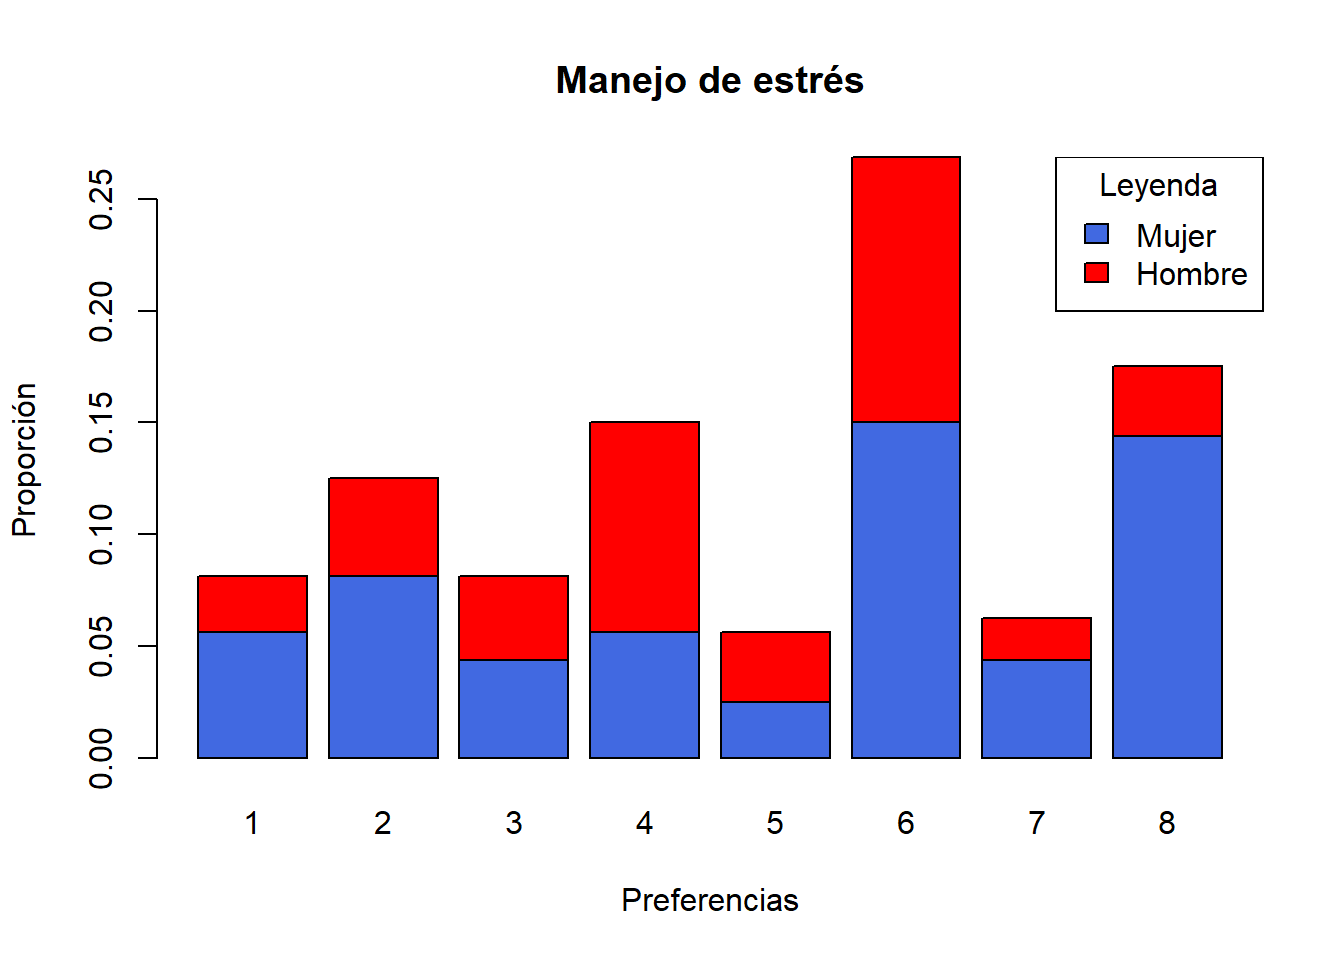
\includegraphics{S7_Informe_files/figure-latex/unnamed-chunk-12-1.pdf}
Durante el periodo estudiado se observa que la incidencia de Deficit de
ganancia de peso tiene sus valores máximos en las DIRESAs de Loreto,
Amazonas y Junin. De esta forma, podemos ver que la región selva
nuevamente predomina en el extremo de maxima incidencia. En la gráfica
se puede observar una dispersión considerable de las incidencias de
déficit, lo cual se confirma con una desviación estándar de 2.62.

\hypertarget{relaciuxf3n-del-estado-nutricional-de-madres-gestantes-y-el-estado-nutricional-de-niuxf1os}{%
\subsection{Relación del estado nutricional de madres gestantes y el
estado nutricional de
niños}\label{relaciuxf3n-del-estado-nutricional-de-madres-gestantes-y-el-estado-nutricional-de-niuxf1os}}

En la siguiente sección se analiza la correlación entre la incidencia de
madres gestantes en déficit nutricional de una DIRESA y el indice de
niños en estado de desnutrición en una misma DIRESA. Cabe destacar que
no todas las DIRESAs evaluados en el estudio de madres gestantes se
encuentran en el estudio de niños y viceverza, por lo que para esta
unión se consideraran únicamente los casos completos.

\begin{Shaded}
\begin{Highlighting}[]
\NormalTok{df\_desnutricion }\OtherTok{\textless{}{-}}\NormalTok{ df\_desges}
\NormalTok{df\_desnutricion }\OtherTok{\textless{}{-}} \FunctionTok{inner\_join}\NormalTok{(df\_desnutricion, df\_desna,}\AttributeTok{by=}\StringTok{"Diresa"}\NormalTok{)}
\NormalTok{df\_desnutricion }\OtherTok{\textless{}{-}} \FunctionTok{inner\_join}\NormalTok{(df\_desnutricion, df\_desnc,}\AttributeTok{by=}\StringTok{"Diresa"}\NormalTok{)}
\NormalTok{df\_desnutricion }\OtherTok{\textless{}{-}} \FunctionTok{inner\_join}\NormalTok{(df\_desnutricion, df\_desng,}\AttributeTok{by=}\StringTok{"Diresa"}\NormalTok{)}
\NormalTok{df\_desnutricion}
\end{Highlighting}
\end{Shaded}

\begin{verbatim}
## # A tibble: 15 x 5
## # Groups:   Diresa [15]
##    Diresa       GestanteDeficit NiñoDesAguda NiñoDesCronica NiñoDesGlobal
##    <chr>                  <dbl>        <dbl>          <dbl>         <dbl>
##  1 AMAZONAS               14.0         1.52           21.5          4.24 
##  2 ANCASH                  5.82        1.19           20.0          3.85 
##  3 AYACUCHO                6.98        1.24           16.0          3.56 
##  4 CUSCO                   5.95        1.51           14.3          3.74 
##  5 HUANCAVELICA            6.97        1.32           23.4          4.59 
##  6 ICA                     6.92        1.42            7.07         1.59 
##  7 JUNIN                  10.6         1.73           16.8          4.52 
##  8 LA LIBERTAD             6.74        1.52           20.2          3.95 
##  9 LAMBAYEQUE              7.14        2.08           16.4          3.28 
## 10 LIMA                    6.76        1.04            9.67         1.86 
## 11 LORETO                 15.1         2.79           21.3          6.95 
## 12 PASCO                   7.89        1.92           16.9          4.37 
## 13 PUNO                    4.93        1.10           12.0          2.52 
## 14 TACNA                   3.27        0.829           3.16         0.567
## 15 TUMBES                  6.83        2.29            7.72         2.78
\end{verbatim}

\hypertarget{relaciuxf3n-con-desnutriciuxf3n-aguda}{%
\subsubsection{Relación con Desnutrición
Aguda}\label{relaciuxf3n-con-desnutriciuxf3n-aguda}}

\begin{verbatim}
## `geom_smooth()` using formula 'y ~ x'
\end{verbatim}

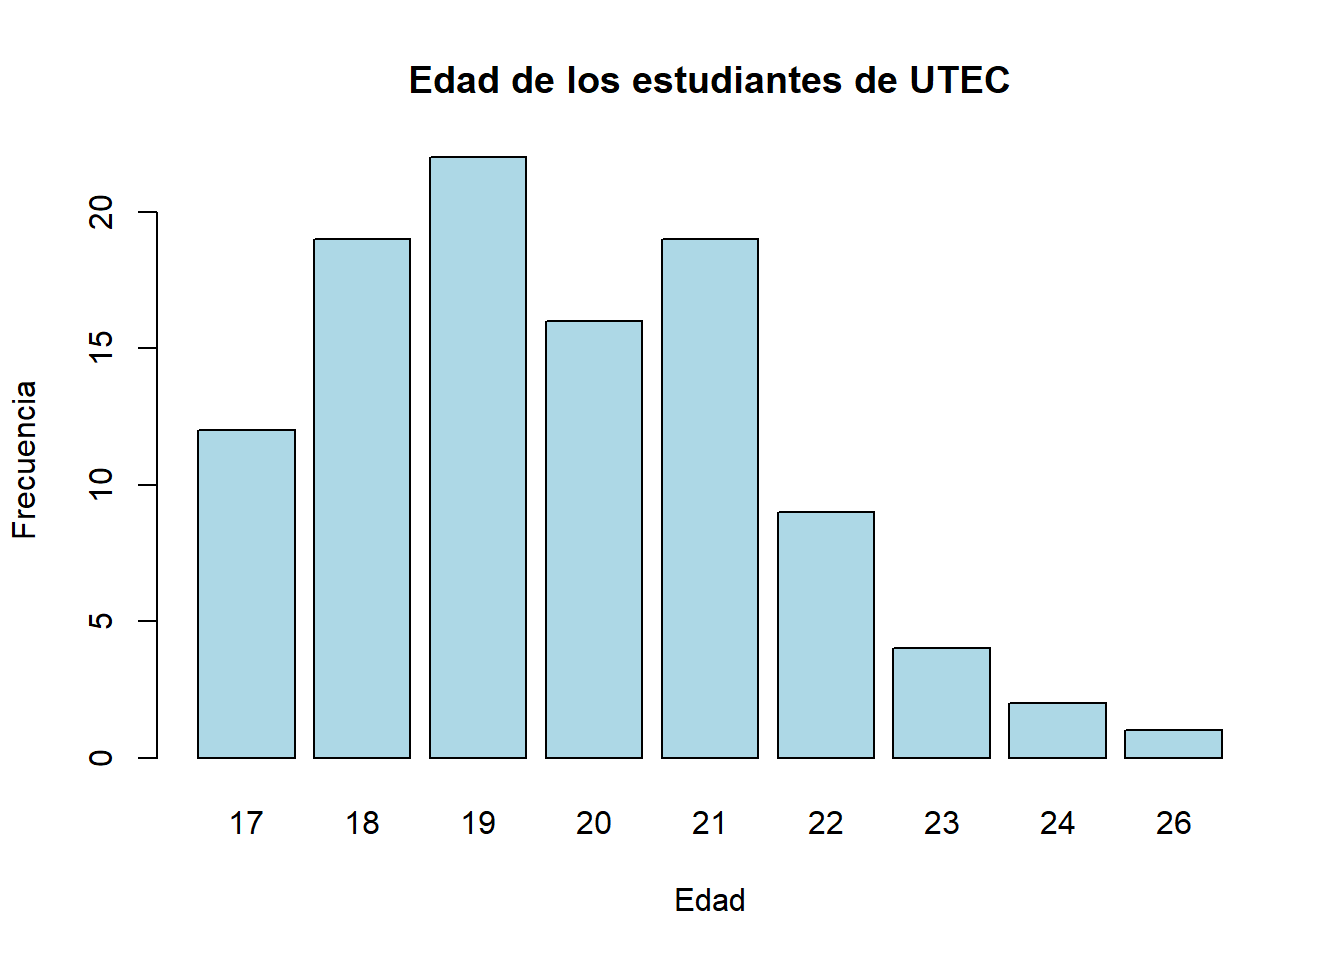
\includegraphics{S7_Informe_files/figure-latex/unnamed-chunk-14-1.pdf}

\begin{verbatim}
## [1] "Correlacion: 0.6381652732388"
\end{verbatim}

Como podemos observar en la gráfica existe una moderada correlación
positiva entre la incidencia de Madres gestantes en deficit nutricional
y la incidencia de niños con desnutrición aguda. Esta relación se puede
confirmar en base al valor obtenido del coeficiente de Pearson, el cual
tiene un valor de 0.64.

\hypertarget{relaciuxf3n-con-desnutriciuxf3n-cronica}{%
\subsubsection{Relación con Desnutrición
Cronica}\label{relaciuxf3n-con-desnutriciuxf3n-cronica}}

\begin{verbatim}
## `geom_smooth()` using formula 'y ~ x'
\end{verbatim}

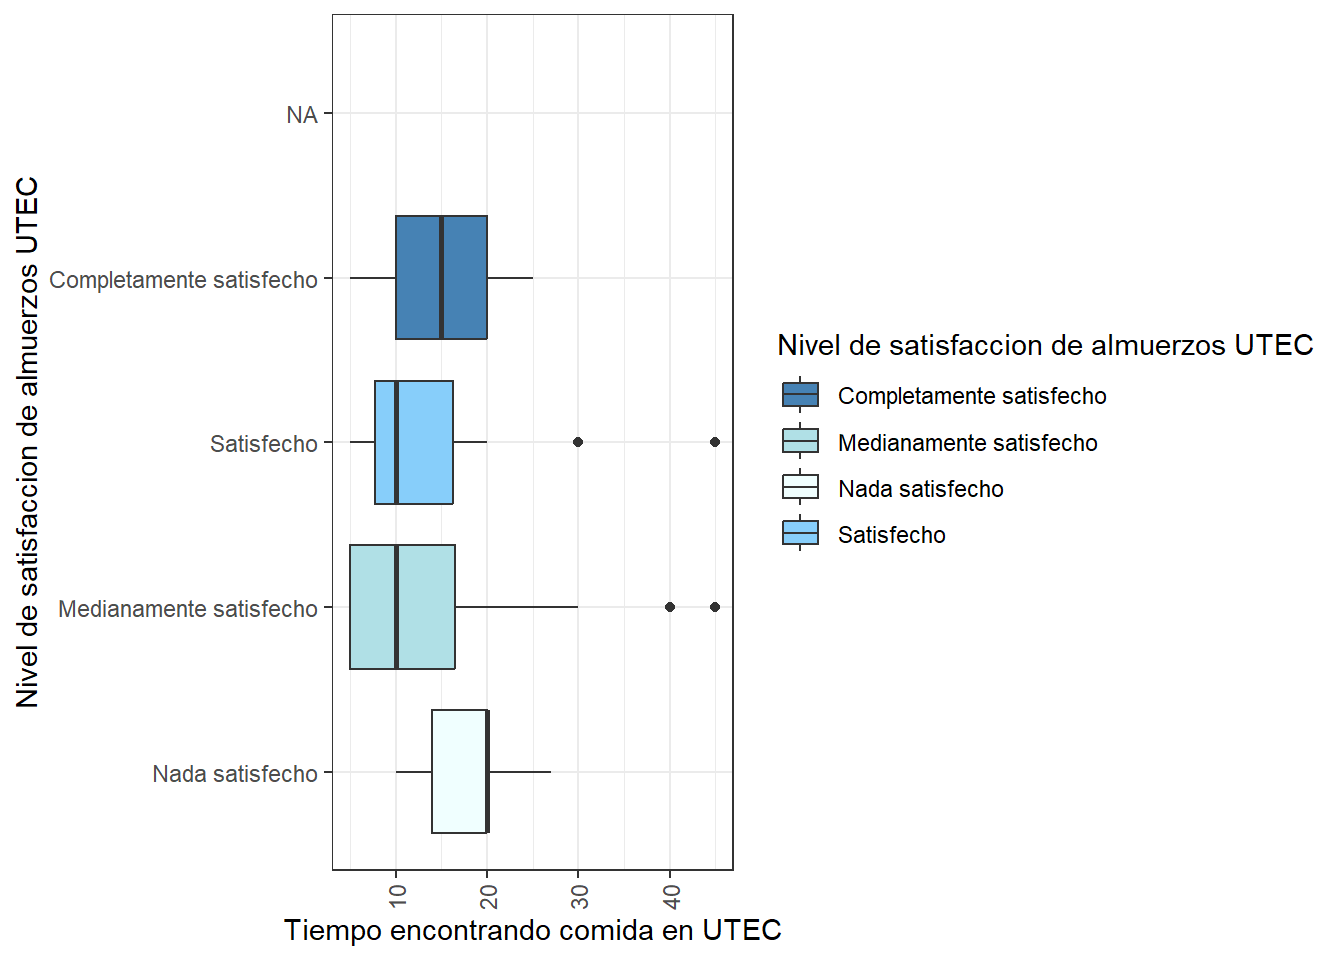
\includegraphics{S7_Informe_files/figure-latex/unnamed-chunk-15-1.pdf}

\begin{verbatim}
## [1] "Correlacion: 0.562652064109414"
\end{verbatim}

Similar a lo que pudimos observar en el primer diagrama de dispersión,
en esta gráfica también podemos observar una moderada correlación
positiva entre la incidencia de madres gestantes en déficit nutricional
y la incidencia de niños con desnutrición crónica. No obstante, al
calcular el coeficiente de Pearson, nos podemos dar cuenta que realmente
esta relación es más débil con un valor de 0.56. Ello se debe en gran
medida al conjunto de datos concentrados entre 6\% y 8\% de madres en
deficit los cuales se encuentran altamente disperso.

\hypertarget{relaciuxf3n-con-desnutriciuxf3n-global}{%
\subsubsection{Relación con Desnutrición
Global}\label{relaciuxf3n-con-desnutriciuxf3n-global}}

\begin{verbatim}
## `geom_smooth()` using formula 'y ~ x'
\end{verbatim}

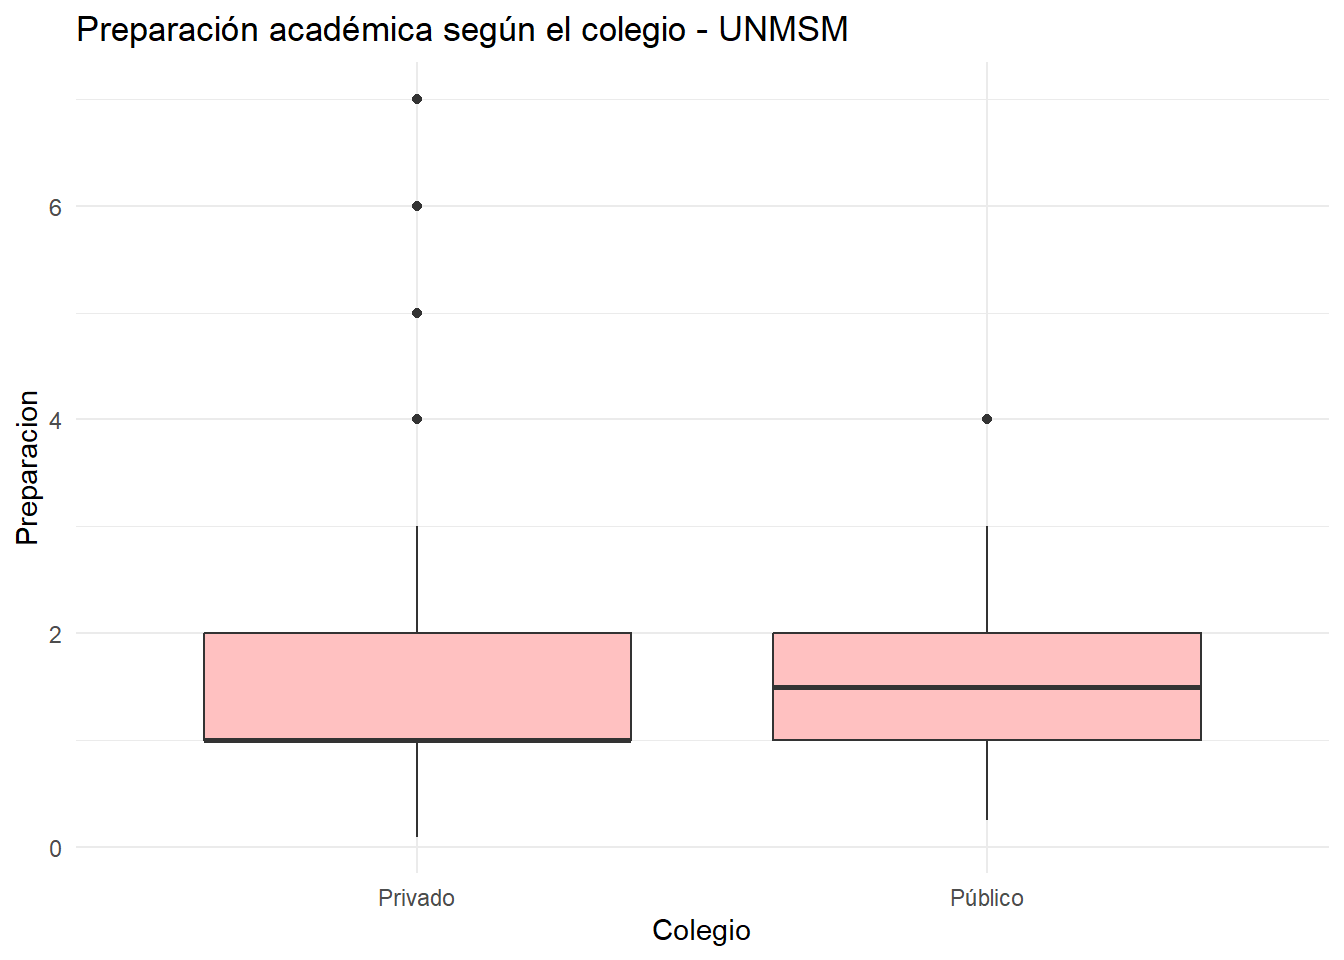
\includegraphics{S7_Informe_files/figure-latex/unnamed-chunk-16-1.pdf}

\begin{verbatim}
## [1] "Correlacion: 0.747173037378099"
\end{verbatim}

En comparación con los graficos previos, este diagrama es el que muestra
la correlación mas fuerte de los tres. Ello se ve reforzado por tener un
coeficiente de Pearson de 0.75, lo que nos indica que es una correlación
fuerte.

\end{document}
